\chapter{Classification}

This section describes the use of a deep neural network to accomplish an end-to-end particle reconstruction task. The model consists of a neural architecture which simultaneously performs both particle classification and energy regression. This combined network is trained using the ECAL and HCAL cell arrays as well as the total ECAL energy and total HCAL energy as inputs. The training loss function is written as the sum of a binary cross entropy for particle identification and a mean-square error loss for energy regression. Through experimentation, we found that multiplying the energy component of the loss function by a factor of 200 gave the best results, as it was easier to quickly achieve low loss values for energy regression.

We compare three different architectures for our reconstruction model, each trained using calorimeter cell-level information as inputs:
\begin{itemize}
\item A dense (i.e, fully connected) neural network (DNN).
\item A 3D convolutional network (CNN).
\item A network based on GoogLeNet (GN)~\cite{GoogLeNet}, using layers of inception modules.
\end{itemize}

In order to compare the model performance to a typical state-of-the-art particle reconstruction algorithm, we also consider the following alternatives:
\begin{itemize}
    \item A feature-based BDT (see Appendix~\ref{app:BDT}) for the classification task.
    \item A linear regression for the regression task.
    \item A BDT for the regression task (for more info on regression baselines see Appendix~\ref{app:regression_baseline}).
\end{itemize}

In a previous study~\cite{NIPS}, we compared the classification accuracy obtained with a neural model taking as input the energy cells, a feature-based neural models, and a feature-based BDTs. In that context, we demonstrated that feature-based BDTs and neural networks perform equally well, and are both equally capable of correctly classify particles from a small set of calculated features. 
%Increases in classification accuracy are mostly due to the neural architecture's ability to extract meaning from a much larger input dataset, the calorimeter cell-level energy information. For this reason, w
We do not compare feature-based neural networks in this paper, and use feature-based BDTs to represent the current state-of-the-art classification algorithms.

\section{Deep Network Models}

The three ML models take as input the ECAL and HCAL 3D energy arrays of the REC dataset (see Section~\ref{sec:data}), together with the total energies recorded in ECAL and in HCAL (i.e., the sum of the values stored in the 3D arrays), as well as the estimated $\phi$ and $\eta$ angles of the incoming particle, calculated using the collision origin and the barycenter of the event. The architecture of each model is defined with a number of floating parameters (e.g. number of hidden layers), which are refined through a hyperparameter optimization, as described in Section~\ref{sec:hpscan}. Each model returns three numbers. After applying a softmax activation, two of these elements are interpreted as the classification probabilities of the current two-class problem. The third output is interpreted as the energy of the particle.

Here we describe in detail the three model architectures:

\begin{itemize}
    \item In the DNN model we first flatten our ECAL and HCAL inputs into 1D arrays. We then concatenate these array along with the total ECAL energy, total HCAL energy, estimated $\phi$, and estimated $\eta$, for an array of total size $25 \times 25 \times 25 + 11 \times 11 \times 60 + 4 = 22889$ inputs. This array is fed as input to the first layer of the DNN, followed by a number of hidden layers each followed by a ReLU activation function and a dropout layer. The number of neurons per hidden layer and the dropout probability are identical for each relevant layer. The number of hidden layers, number of hidden neurons per layer, and dropout rate are hyperparameters, tuned as described in the next session.  Finally, we take the output from the last dropout layer, append the total energies and estimated angles again, and feed the concatenated array into a final hidden layer, which results in a three-element output. 
    \item The CNN architecture consists of one 3D convolutional layer for each of the ECAL and HCAL inputs, each followed by a ReLU activation function and a max pooling layer of kernel size $2 \times 2 \times 2$. The number of filters and the kernel size in the ECAL convolutional layer are treated as optimized hyperparameter (see next session). The HCAL layer is fixed at 3 filters with a kernel size of $2 \times 2 \times 6$. The two outputs are then flattened and concatenated along with the total ECAL and HCAL energies, as well as the estimated $\phi$ and $\eta$ coordinates of the incoming particle. The resulting 1D array is passed to a sequence of dense layers each followed by a ReLU activation function and dropout layer, as in the DNN model. The number of hidden layers and the number of neurons on each layer are considered as hyperparameters to be optimized. The output layer consists of three numbers, as for the DNN model. We found that adding additional convolutional layers to this model beyond the first had little impact on performance. This may be because a single layer is already able to capture important information about localized shower structure, and reduces the dimensionality of the event enough where a densely connected net is able to do the rest.
    \item The third model uses elements of the GoogLeNet~\cite{GoogLeNet} architecture. This network processes the ECAL input array with a 3D convolutional layer with 192 filters, a kernel size of 3 in all directions, and a stride size of 1. The result is batch-normalized and sent through a ReLU activation function. This is followed by a series of inception and MaxPool~\cite{conv} layers of various sizes, with the full architecture described in Appendix~\ref{app:GoogLeNet}. The output of this sequence is concatenated to the total ECAL energy, the total HCAL energy, the estimated $\phi$ and $\eta$ coordinates, and passed to a series of dense layers like in the DNN architecture, to return the final three outputs. The number of neurons in the final dense hidden layer is the only architecture-related hyperparameter for the GN model. Due to practical limitations imposed by memory constraints, this model does not take the HCAL 3D array as input. This limitation has a small impact on the model performance, since the ECAL array carries the majority of the relevant information for the problems at hand (see Appendix~\ref{app:classification_HCAL}).
\end{itemize}

On all models, the regression task is facilitated by using skip connections to directly append the input total ECAL and HCAL energies to the last layer. The impact of this architecture choice on regression performance is described in Appendix~\ref{app:skip_connections}. In addition to using total energies, we also tested the possibility of using 2D projections of the input energy arrays, summing along the $z$ dimension (detector depth). This choice resulted in worse performance (see Appendix~\ref{app:z_sum_regression}) and was discarded.

\subsection*{GoogLeNet Model Architecture Details}\label{app:GoogLeNet}

In our GoogLeNet architecture, we use inception modules. In these modules, inputs go through four separate branches and are then concatenated together. For an inception layer denoted as Inception(A, B, C, D, E, F, G) the branches are defined as follows:

\begin{itemize}
    \item Branch 1: A simple $1 \times 1 \times 1$ convolution, taking A input channels to B output channels. This is followed by a batch normalization and a ReLU activation function.
    \item Branch 2: A $1 \times 1 \times 1$ convolution followed by a $3 \times 3 \times 3$ convolution. The first convolution takes A input channels to C output channels, followed by batch normalization and ReLU. This then goes to the next convolution layer, which outputs D channels using a kernel of size $3 \times 3 \times 3$. This is again followed by batch normalization and ReLU.
    \item Branch 3: A $1 \times 1 \times 1$ convolution followed by a $5 \times 5 \times 5$ convolution. The details are the same as for the other branches, but the first convolution takes A input channels to E output channels, and the next convolution outputs F channels.
    \item Branch 4: A max pool of kernel size $3 \times 3 \times 3$ is followed by a convolution of kernel size $1 \times 1 \times 1$ that takes A input channels to G output channels. This is followed once again by batch normalization and ReLU.
\end{itemize}

Here are full details for each layer of the GoogLeNet-based architecture:

\begin{itemize}
    \item Apply instance normalization to ECAL input.
    \item Convolution with 3D kernel of size 3, going from 1 input channel to 192 channels, with a padding of 1. This is followed by batch normalization and ReLU.
    \item Inception(192,  64,  96, 128, 16, 32, 32)
    \item Inception(256, 128, 128, 192, 32, 96, 64)
    \item Max pooling with a 3D kernel of size 3, a stride of 2, and padding of 1.
    \item Inception(480, 192,  96, 208, 16,  48,  64)
    \item Inception(512, 160, 112, 224, 24,  64,  64)
    \item Inception(512, 128, 128, 256, 24,  64,  64)
    \item Inception(512, 112, 144, 288, 32,  64,  64)
    \item Inception(528, 256, 160, 320, 32, 128, 128)
    \item Max pooling with a 3D kernel of size 3, a stride of 2, and padding of 1.
    \item Inception(832, 256, 160, 320, 32, 128, 128)
    \item Inception(832, 384, 192, 384, 48, 128, 128)
    \item Average pooling with a 3D kernel of size 7 and a stride of 1.
    \item The output array is flattened and concatenated with input $\phi$, $\eta$, total ECAL energy, and total HCAL energy.
    \item A densely connected layer with 1024 outputs, followed by ReLU.
    \item The output array is once again concatenated with the same input values.
    \item A final densely connected layer outputs 5 values, as in the architectures of the other two models.
\end{itemize}

The full architecture is shown in Figure~\ref{fig:gn_with_inceptin}.

\begin{figure}[htbp]
\centering
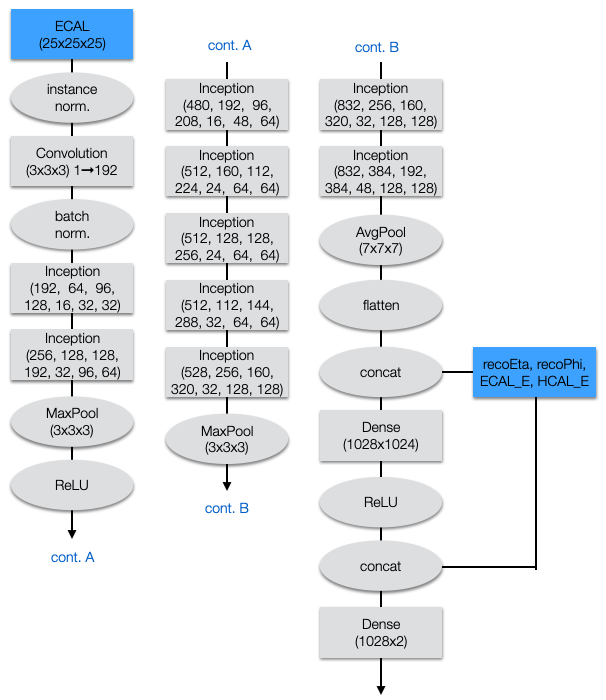
\includegraphics[width=0.38\textwidth]{Images/Calo/GN_architecture.png}
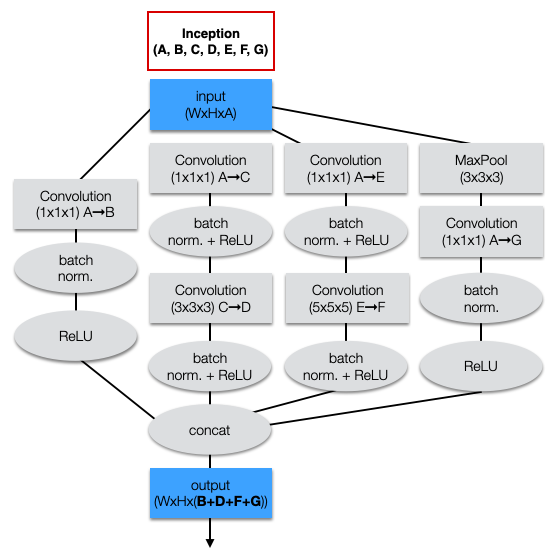
\includegraphics[width=0.38\textwidth]{Images/Calo/inception_architecture.png}
\caption{GoogLeNet-based architecture (top) and component inception architecture (bottom).
}
\label{fig:gn_with_inceptin}
\end{figure}

\subsection*{Use of HCAL in Classification}\label{app:classification_HCAL}

Since the GoogLeNet architecture was quite large and required significant memory usage and computational power, we decided to investigate the possibility of leaving out HCAL cell-level information, since most of the particle shower occurs in the ECAL. Using our best-performing DNN architecture, we ran ten training sessions with HCAL information, and ten training sessions without HCAL. Averaged training curves from these runs are shown in Figures~\ref{fig:HCAL_study_elechpi} and~\ref{fig:HCAL_study_gammapi0}. These studies demonstrated that including the HCAL caused little to no improvement in classification accuracy. For memory purposes, we thus kept HCAL cell-level information out of our GN architecture. Summed HCAL energy was still fed as an input to the combined classification-regression net, for use in energy regression.

We must note here that though HCAL information is useful for particle reconstruction in general, the reason we do not see much use for it here is because we are mostly looking at events where the majority of energy is deposited in the ECAL. This is particularly true due to the HCAL/ECAL ratio we have applied to electron/charged pion events.

\begin{figure}[htbp]
\centering
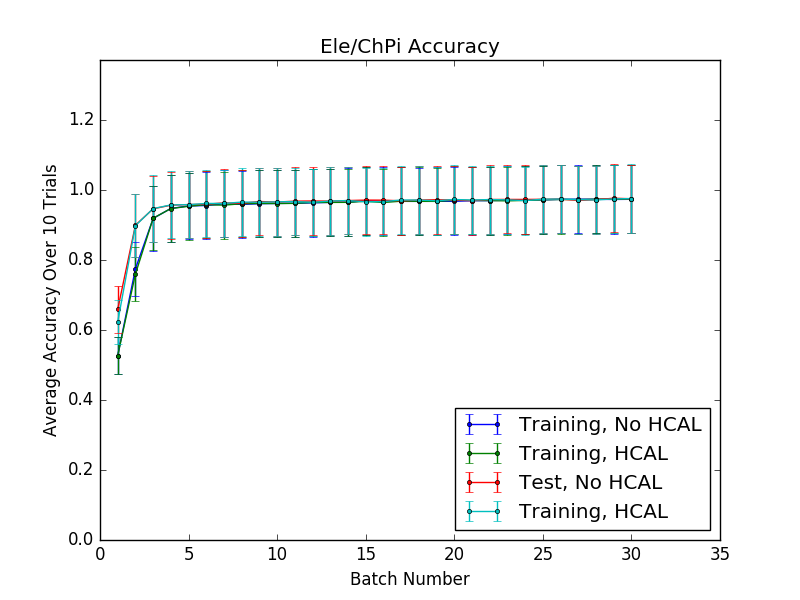
\includegraphics[width=0.38\textwidth]{Images/Calo/HCAL_study_elechpi_accuracy.png}
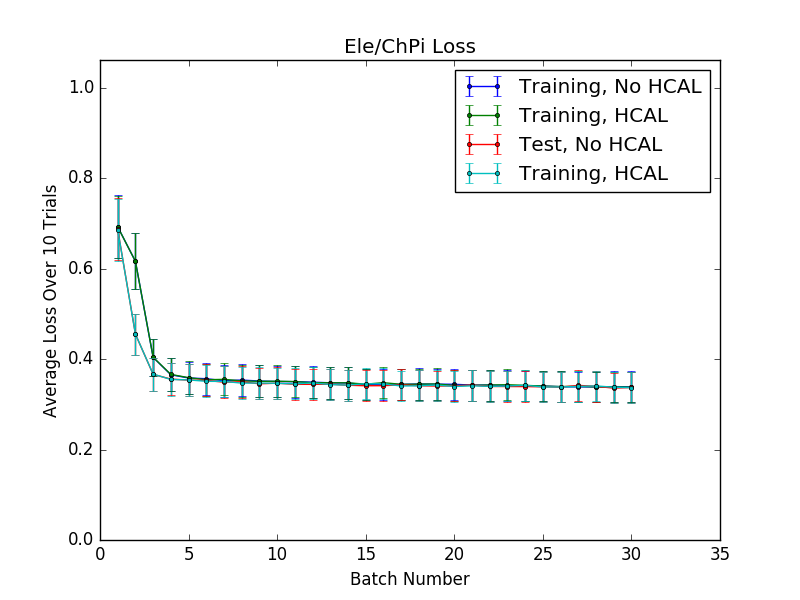
\includegraphics[width=0.38\textwidth]{Images/Calo/HCAL_study_elechpi_loss.png}
\caption{Accuracy and loss curves for electron/charged pion classification, with and without HCAL cells, using best DNN architecture.}
\label{fig:HCAL_study_elechpi}
\end{figure}

\begin{figure}[htbp]
\centering
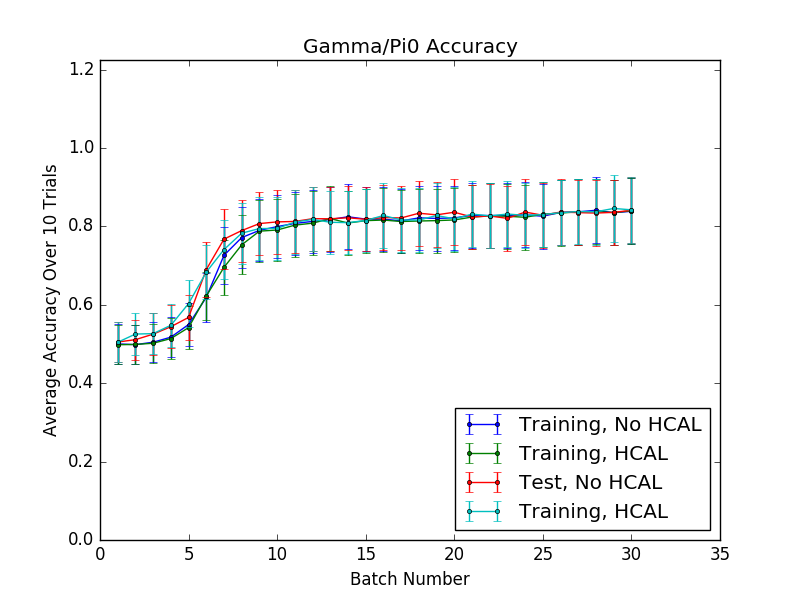
\includegraphics[width=0.38\textwidth]{Images/Calo/HCAL_study_gammapi0_accuracy.png}
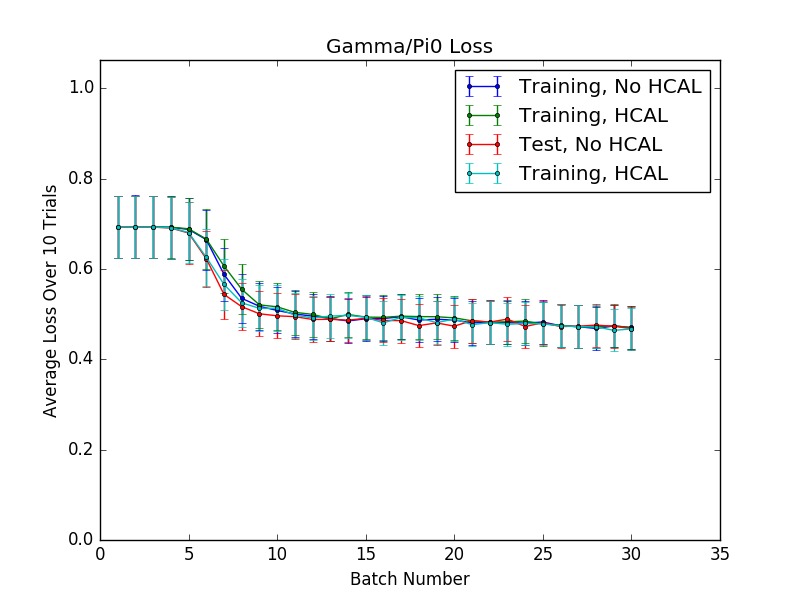
\includegraphics[width=0.38\textwidth]{Images/Calo/HCAL_study_gammapi0_loss.png}
\caption{Accuracy and loss curves for photon/neutral pion classification, with and without HCAL cells, using best DNN architecture.}
\label{fig:HCAL_study_gammapi0}
\end{figure}

\section{Hyperparameter Scans}
\label{sec:hpscan}

In order to determine the best architectures for the end-to-end reconstruction models, we scanned over a hyperparameter space for each architecture. Learning rate and decay rate were additional hyperparameters for each architecture. For simplicity, we used classification accuracy for the $\gamma$ vs. $\pi^0$ problem as a metric to determine the overall best hyperparameter set for each architecture. This is because a model optimized for this task was found to generate good results for the other three tasks as well, and because $\gamma$ vs. $\pi^0$ classification was found to be the most difficult problem.

Training was performed at each hyperparameter point ten times, in order to obtain an estimate of the uncertainty associated with each quoted performance value. For each scan point, the DNN and CNN architectures trained on 400,000 events, using another sample of 400,000 events for testing. DNN and CNN scan points trained for three epochs each, taking about seven hours each. GN trained on 100,000 events and tested on another 100,000. Due to a higher training time, each GN scan point only trained for a single epoch, taking about twenty hours.

For CNN and DNN training, we used batches of 1,000 events when training. However, due to GPU memory limitations, we could not do the same with GN. Instead, we split each batch into 100 minibatches of ten events each. A single minibatch was loaded on the GPU at a time, and gradients were added up after back-propagation. We waited until after each batch was fully calculated to update network weights using the combined gradients.

The best settings were found to be as follows:
\begin{itemize}
    \item For DNN, 4 hidden layers, 512 neurons per hidden layer, a learning rate of 0.0002, decay rate of 0, and a dropout probability of 0.04.
    \item For CNN, 4 hidden layers and 512 neurons per hidden layer, a learning rate of 0.0004, decay rate of 0, a dropout probability of 0.12, 6 ECAL filters with a kernel size of $6 \times 6 \times 6$.
    \item For GN, 1024 neurons in the hidden layer, 0.0001 learning rate, and 0.01 decay rate. 
\end{itemize}
%For CNN and GN, a very mild dependence on the number of neurons per hidden layer is observed. 

\begin{figure*}[htbp]
\centering
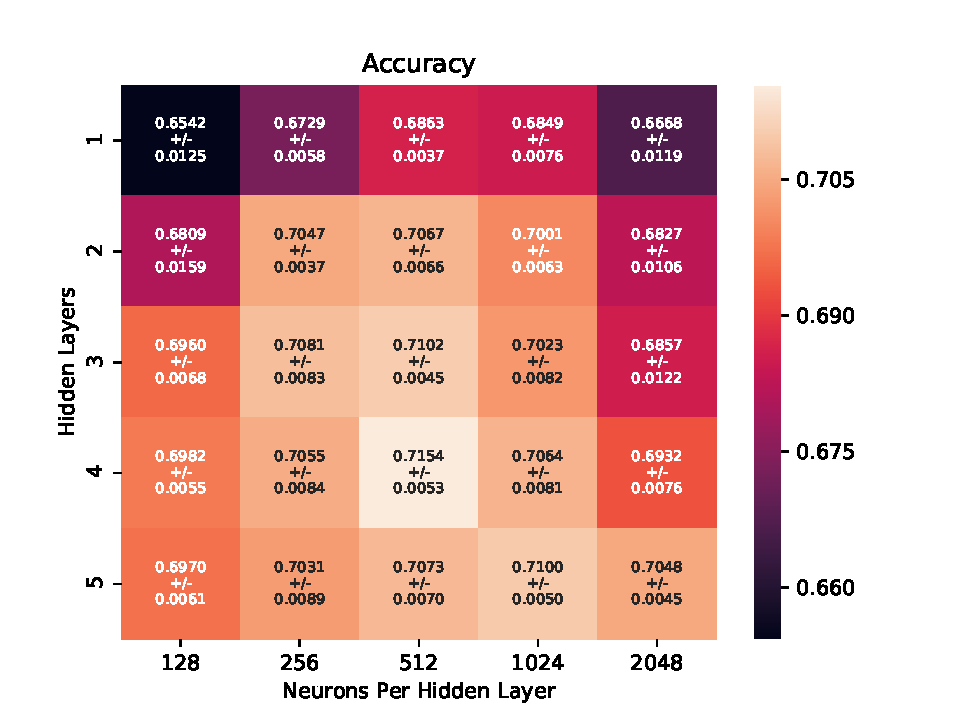
\includegraphics[width=0.45\textwidth]{Images/Calo/DNN_hl_nhl.pdf}
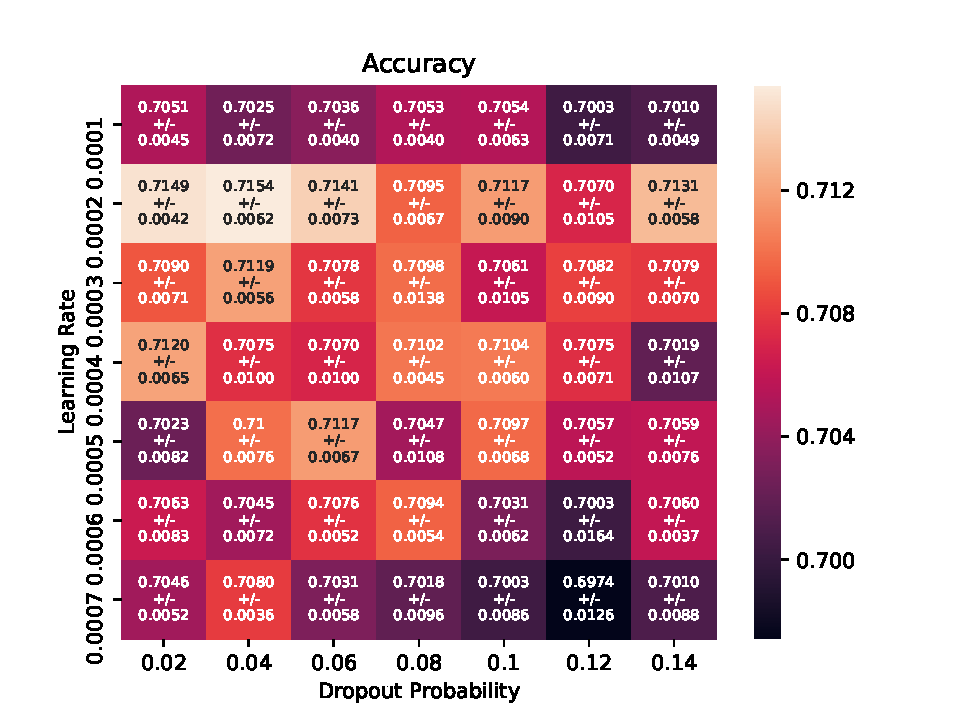
\includegraphics[width=0.45\textwidth]{Images/Calo/DNN_lr_dp.pdf} \\
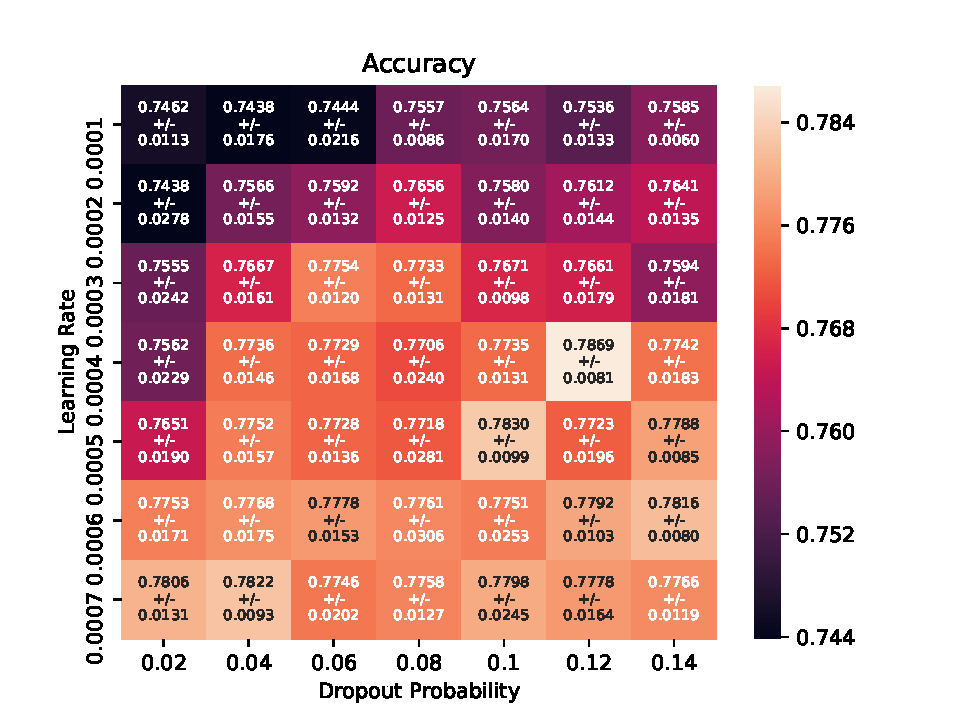
\includegraphics[width=0.45\textwidth]{Images/Calo/CNN_lr_dp.pdf}
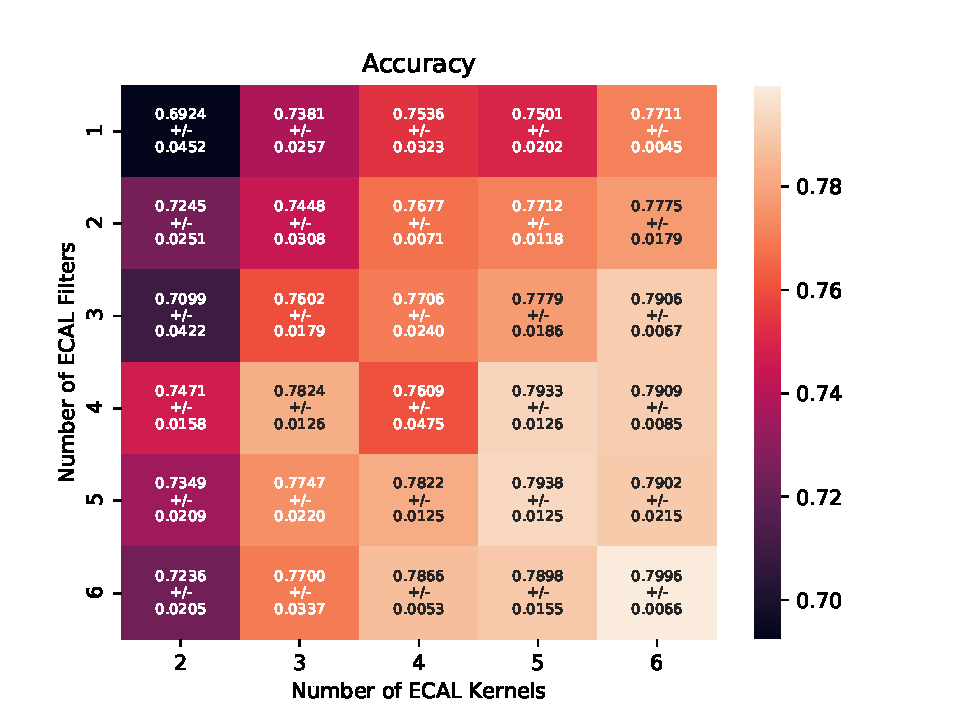
\includegraphics[width=0.45\textwidth]{Images/Calo/CNN_nECALfilt_nECALkern.pdf} \\
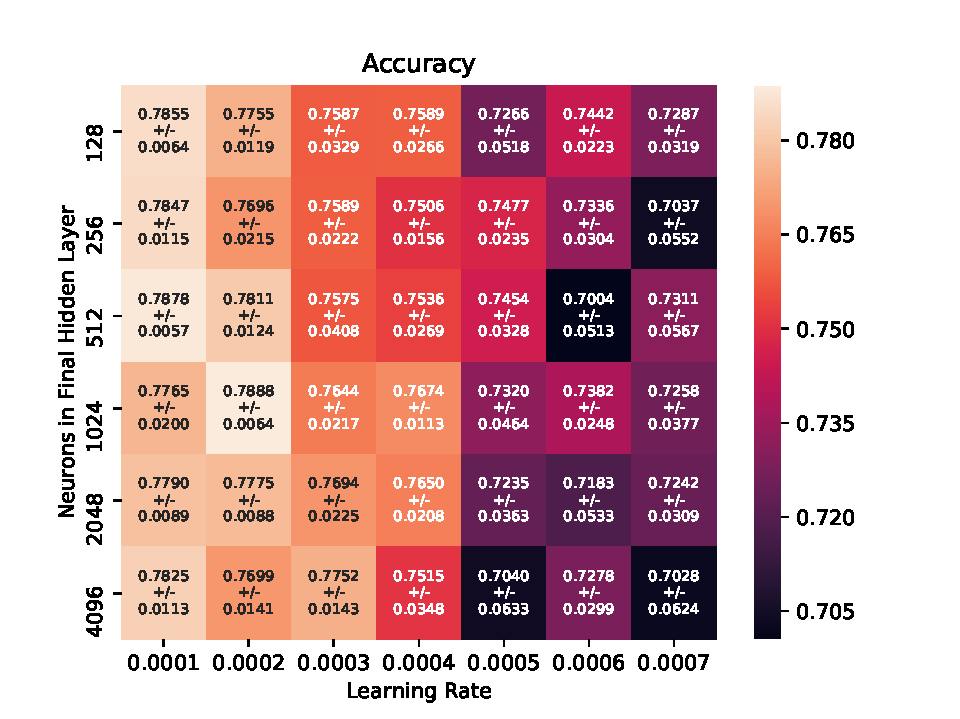
\includegraphics[width=0.45\textwidth]{Images/Calo/GN_nhl_lr.pdf}
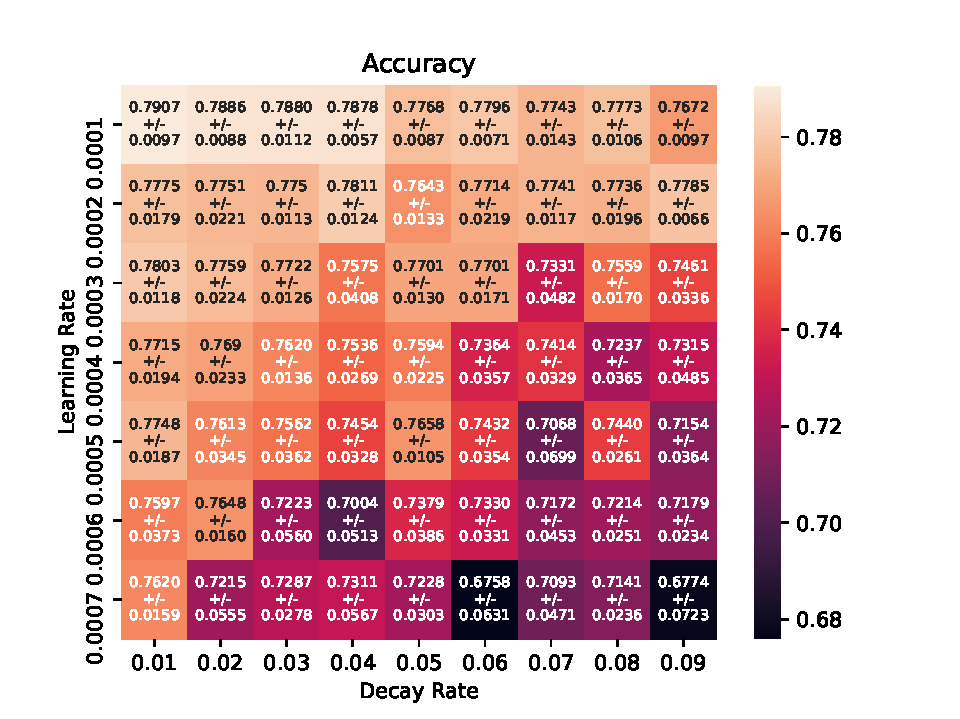
\includegraphics[width=0.45\textwidth]{Images/Calo/GN_lr_dr.pdf}
\caption{Selected hyperparameter scan results for DNN (top), CNN (center), and the GoogLeNet-based architecture (bottom). In each figure, the classification accuracy is displayed as a function of the hyperparameters reported on the two axes.}
\label{fig:scan_hyperparameter}
\end{figure*}

The DNN, CNN, and GN-based models had 9823774 ($\sim$10M), 3003692 ($\sim$3M), and 14956286 ($\sim$15M) trainable parameters respectively after the hyperparameter scans.

Selected hyperparameter scan slices are shown in Figure~\ref{fig:scan_hyperparameter}. 
These 2D scans were obtained setting all values besides the two under consideration (i.e., those on the axes) to be fixed at default values: a dropout rate of 0.08, a learning rate of 0.0004, a decay rate of 0.04, three dense layers for CNN and DNN, and 512 neurons per hidden layer. For GN, the default number of ECAL filters was 3, with a kernel size of 4.
%An ECAL window size of 25 was used in all instances, to allow fair comparison between DNN, CNN, and GN, as larger ECAL sizes posed a memory problem when training GN.

After performing the hyperparameter scan, we trained each architecture using its optimal hyperparameters for a greater number of epochs. The evolution of the training and validation accuracy as a function of the batch number for these extended trainings is shown in Figure~\ref{fig:training_curves_comparison_gamma_pi0}.

\begin{figure}[htbp]
\centering
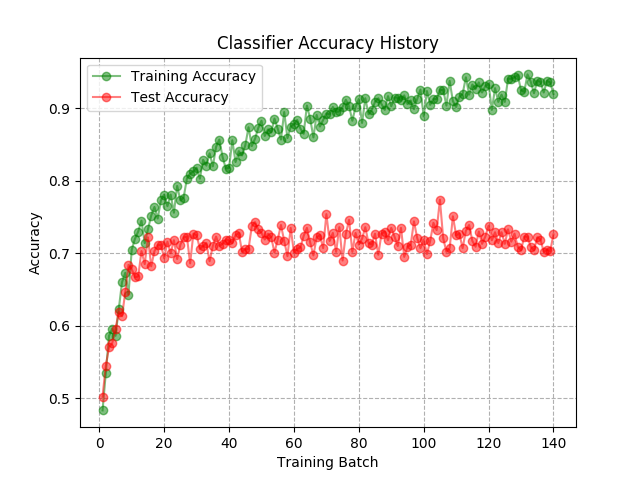
\includegraphics[width=0.42\textwidth]{Images/Calo/DNN_accuracy_batches_long.png}
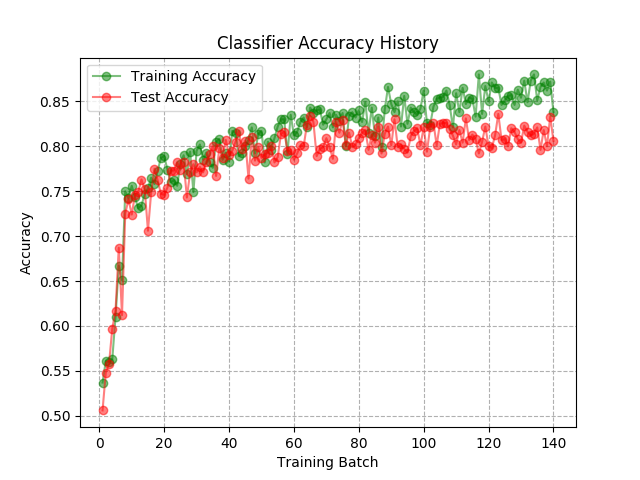
\includegraphics[width=0.42\textwidth]{Images/Calo/CNN_accuracy_batches_long.png}
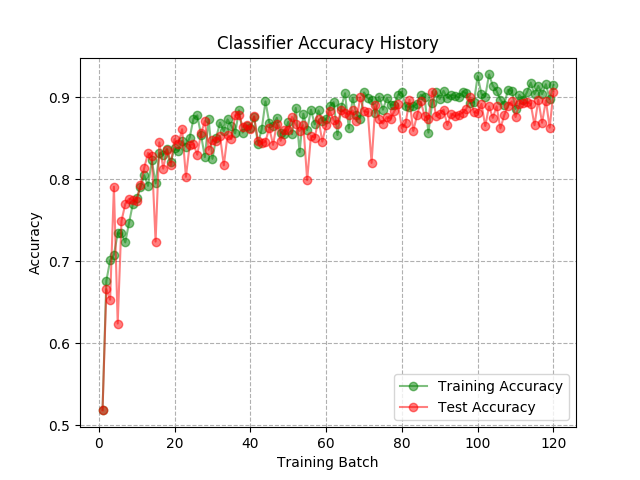
\includegraphics[width=0.42\textwidth]{Images/Calo/GN_accuracy_batches_long.png}
\caption{Training curves for best DNN (top), CNN (middle), and GoogLeNet (bottom) hyperparameters, trained on variable-angle $\gamma$/$\pi^0$ samples. We see that the DNN over-trains quickly and saturates at a relatively low accuracy, while the CNN takes longer to over-train and reaches a higher accuracy, and GoogLeNet performs best of all. Each 400 batches corresponds to a single epoch.}
\label{fig:training_curves_comparison_gamma_pi0}
\end{figure}

\section{Results}

We apply the best architectures described in the previous section separately to our electron vs. charged pion and photon vs. neutral pion reconstruction problems.

Figure~\ref{fig:architectures_ROC_comparisons} shows ROC curve comparisons for the two classification tasks. As expected, the electron vs. charged pion classification problem was found to be a simple task, resulting in an area under the curve (AUC) close to $100\%$. For a baseline comparison, the curve obtained for a BDT (see Appendix~\ref{app:BDT}) is also shown. This BDT was optimized using the {\it scikit-optimize} package~\cite{skopt}, and was trained using high-level features computed from the raw 3D arrays. It represents the performance of current (non-deep-learning) ML approaches on these problems.

\begin{figure}[htbp]
\centering
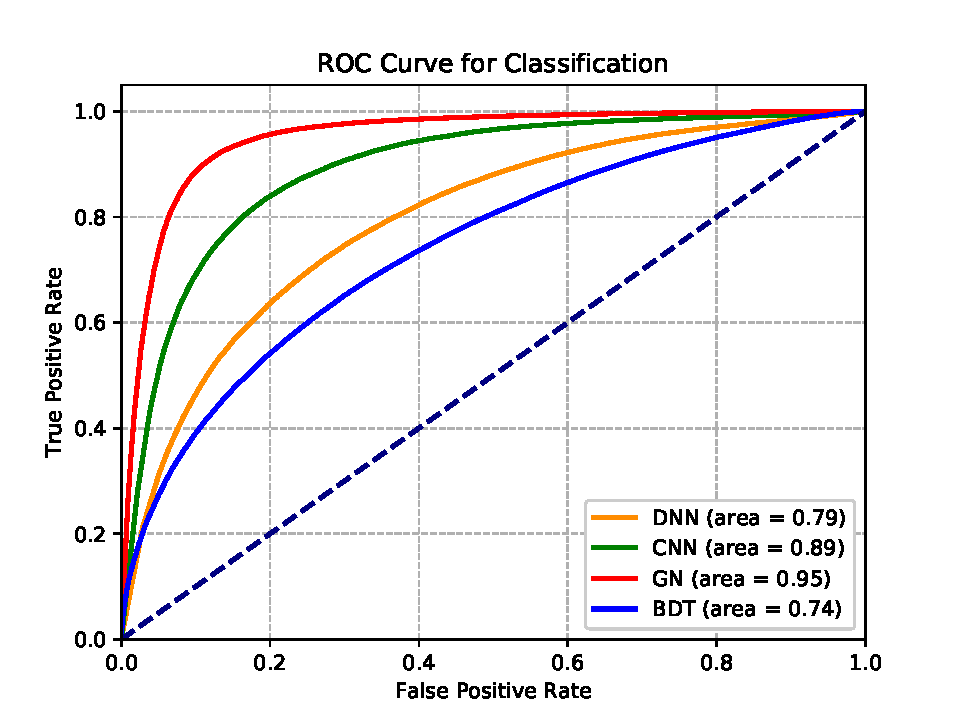
\includegraphics[width=0.45\textwidth]{Images/Calo/architectures_ROC_comparison_gamma_pi0_long.pdf}
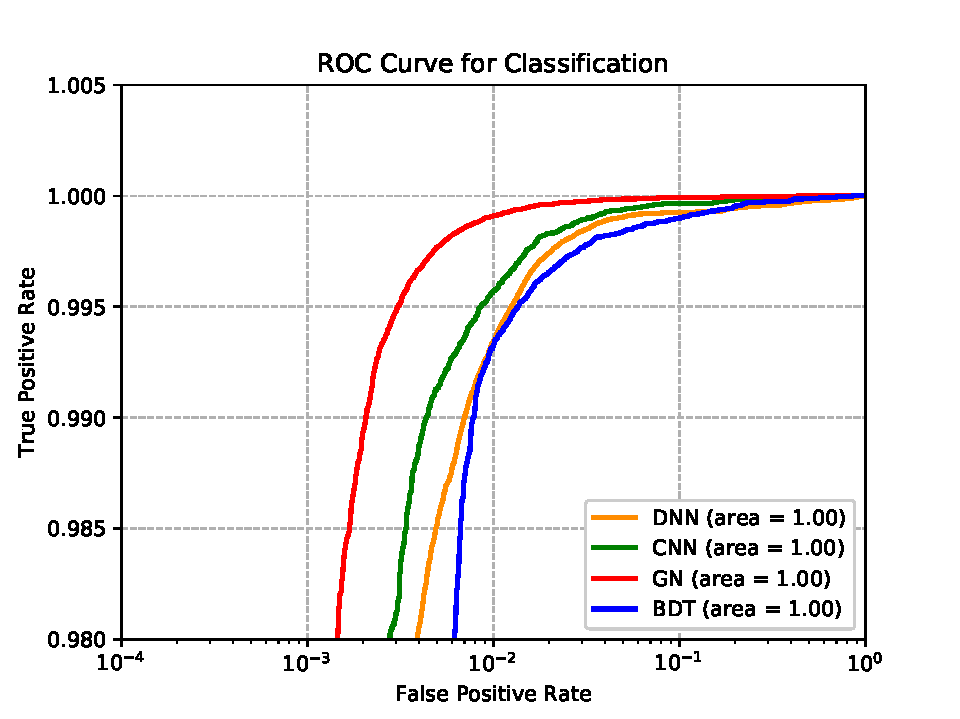
\includegraphics[width=0.45\textwidth]{Images/Calo/architectures_ROC_comparison_ele_chpi_xlog.pdf}
\caption{ROC curve comparisons for $\gamma$ vs. $\pi^0$ (top) and $e$ vs. $\pi^\pm$ (bottom) classification using DNN, CNN, BDT, and GoogLeNet (GN). Samples include particle energies from 2 to 500 GeV, and an inclusive $\eta$ range.}
\label{fig:architectures_ROC_comparisons}
\end{figure}

Our deep learning models outperform the BDT, with the GN reaching the best classification performance on both problems. Figure~\ref{fig:accuracy_bins} shows the best-model performance as a function of the energy and $\eta$ of the incoming particle, for the photon vs. neutral pion and the electron vs. charged pion problems. These figures show that classification accuracy is maintained over a wide range of particle energies and angles. The models appear to perform a bit worse at higher energies for the photon vs. neutral pion case, due to the fact that the pion to two photon decay becomes increasingly collimated at higher energies. Similarly, the performance is slightly worse when particles impact the detector perpendicularly than when they enter at a wide angle, because the shower cross section on the calorimeter inner surface is reduced at $90^{\mathrm o}$, making it harder to distinguish shower features.

\begin{figure*}[htbp]
\centering
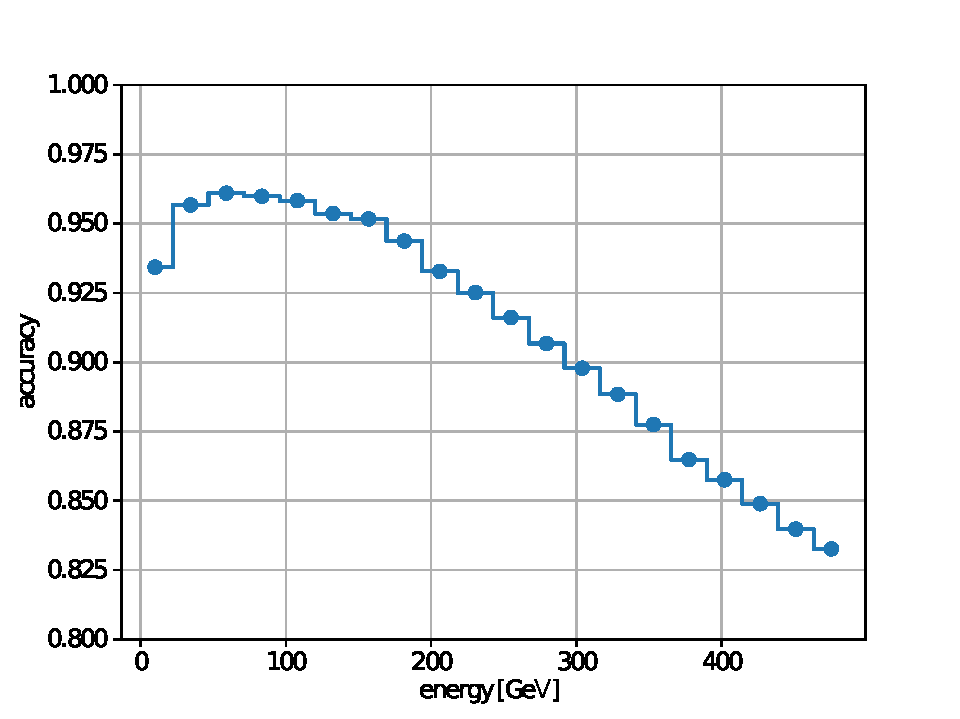
\includegraphics[width=0.45\textwidth]{Images/Calo/gamma_pi0_accuracy_energy_bins.pdf}
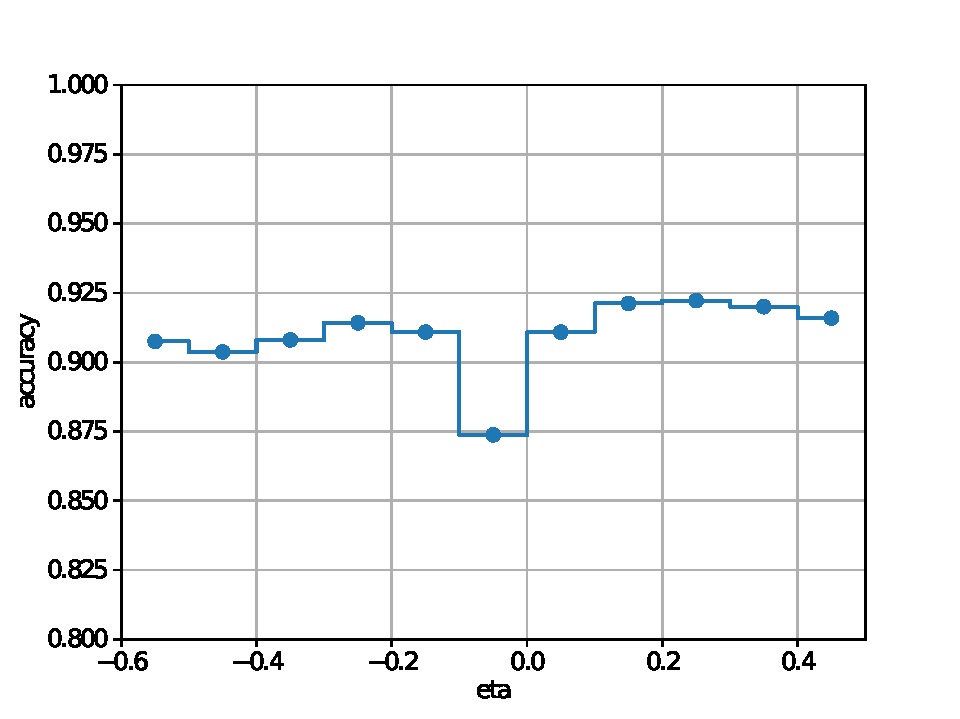
\includegraphics[width=0.45\textwidth]{Images/Calo/gamma_pi0_accuracy_eta_bins.pdf} \\
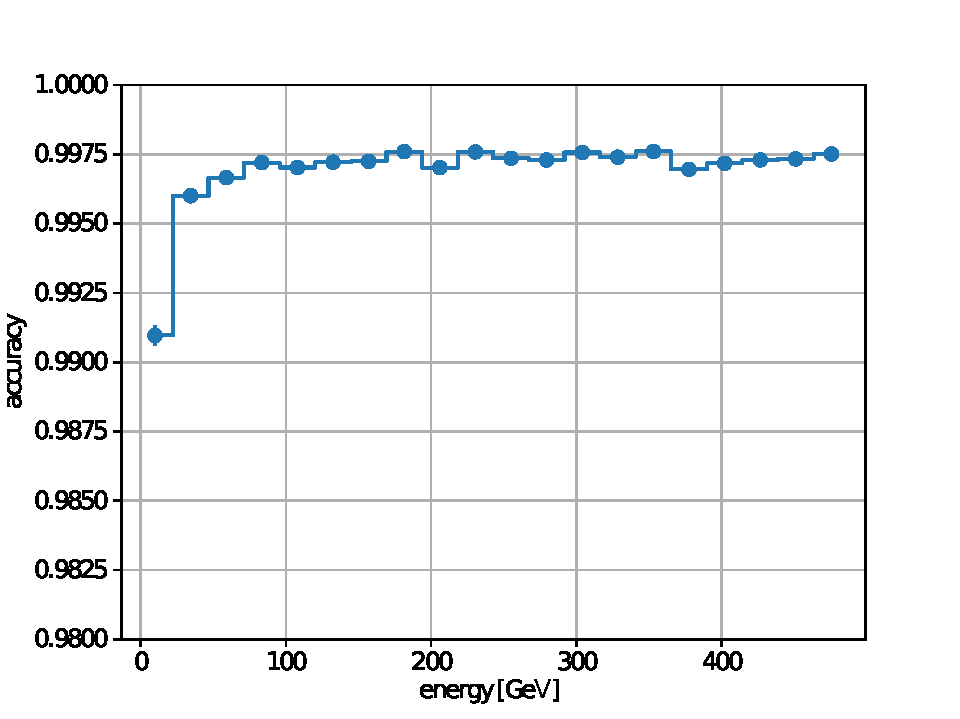
\includegraphics[width=0.45\textwidth]{Images/Calo/ele_chpi_accuracy_energy_bins.pdf}
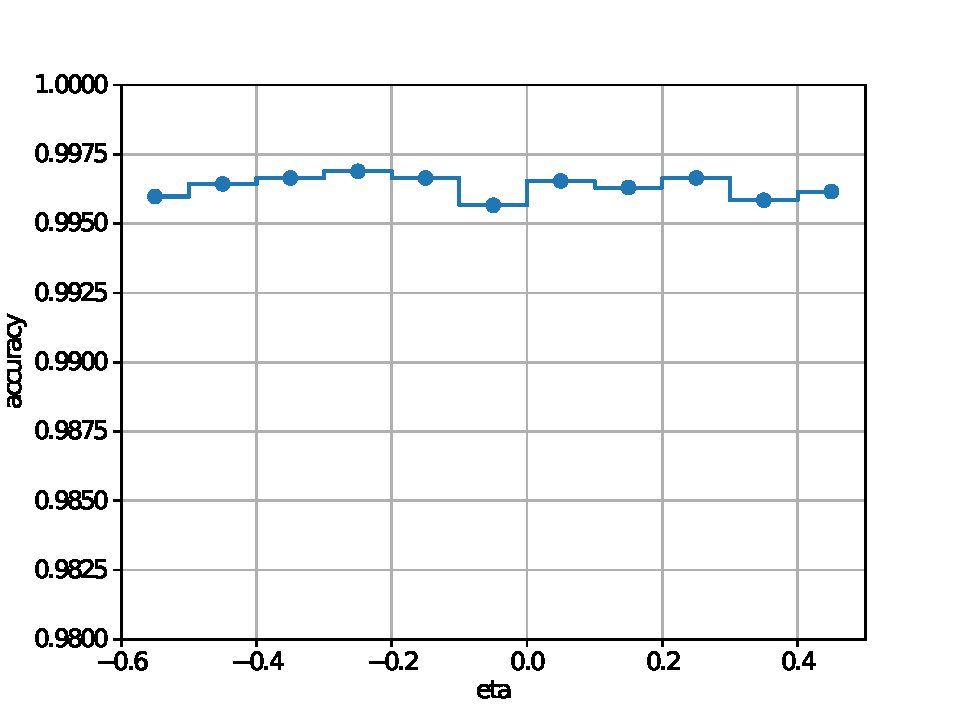
\includegraphics[width=0.45\textwidth]{Images/Calo/ele_chpi_accuracy_eta_bins.pdf}
\caption{Classification accuracy of best performing network for $\gamma$ vs. $\pi^0$ (top) and $e$ vs. $\pi^\pm$ (bottom), in bins of energy (left) and $\eta$ (right).}
\label{fig:accuracy_bins}
\end{figure*}